\chapter{Introduction to routing schemes}

Routing is one of the most fundamental problems in the area of distributed
networking. The goal in this problem is to find a distributed algorithm that
allows any source vertex $v$ in a network $G=(V,E,\omega)$ to route messages
to any destination vertex $u$, where $u, v\in V$.

Each node $v \in V$ is given a unique name with $O(log\; n)$ bits. Also
for each vertex, each outgoing edge is given a unique port number in
$\{1,\dots,deg(v)\}$.

Formally, a routing scheme is comprised of two phases. The first phase is
called the preprocessing phase. In this phase $G$ is preprocessed and the
derived routing information is stored locally with the relevant vertices.

In the second phase - the routing phase - the routing scheme allows any vertex
to route messages to any vertex in a distributed manner only based on the
label of the destination vertex.

A naive approach to routing, is to preprocess a graph by running a SSSP
algorithm from each vertex $v \in V$ and at each vertex $v$ store a hashmap
mapping any vertex in $V$ to a port number.

In the routing phase a vertex will only need to look at the destination label
of the message. If the destination label match the one of the vertex then we
are done, otherwise we lookup what forwarding port for the destination vertex
and forwarding the message.

This approach will ensure a routing of stretch-1 (a min cost path) and the lookup performed at
each vertex can be done in constant time. But this approach will use a lot of
space as each vertex will store a hashmap with $n$ entries where each key is a
destination label using $O(log(n))$ bit.

Thus the space consumed at each node is $\Omega (n\; log\; n)$. This space
complexity renders our naive approach useless as we can not scale it.

In order to reduce memory and ensure for routing costs that are proportional
to distances, there are two parameters that routing schemes try to minimize.
\begin{description}
  \item[Stretch] The max ratio over all source-destination pairs between the
      cost of the path taken by the routing scheme and the cost of a min
      cost path.
  \item[Memory] The max number of bits over all nodes stored for the routing
      scheme. (balanced is preferred)
\end{description}
This article presents a routing scheme that uses $\tilde{O}(\sqrt(n))$
routing table space per vertex, and routes along paths of stretch-3.

\section*{Labeled Routing or Name-Independent Routing}
In the literature we distinguish between \emph{labeled routing} or
\emph{name-independent routing}. To illustrate the differences lets look at a
grid and imagine that the intersections is vertices and the lines are edges.

In labeled routing we are allowed to label the vertices ourself. This allows
us to give every vertex a label representing the $(x,y)$-coordinate of that
vertex. This way we encode topological information into the label names and we
can easily navigate in the graph by forwarding messages to desired port. In
this scenario the available ports for each vertex would be a subset of $\{+y,
-y, +x, -x\}$. \autoref{fig:labeledrouting} illustrates this scenario.
\begin{figure}[htbp]
    \centering
    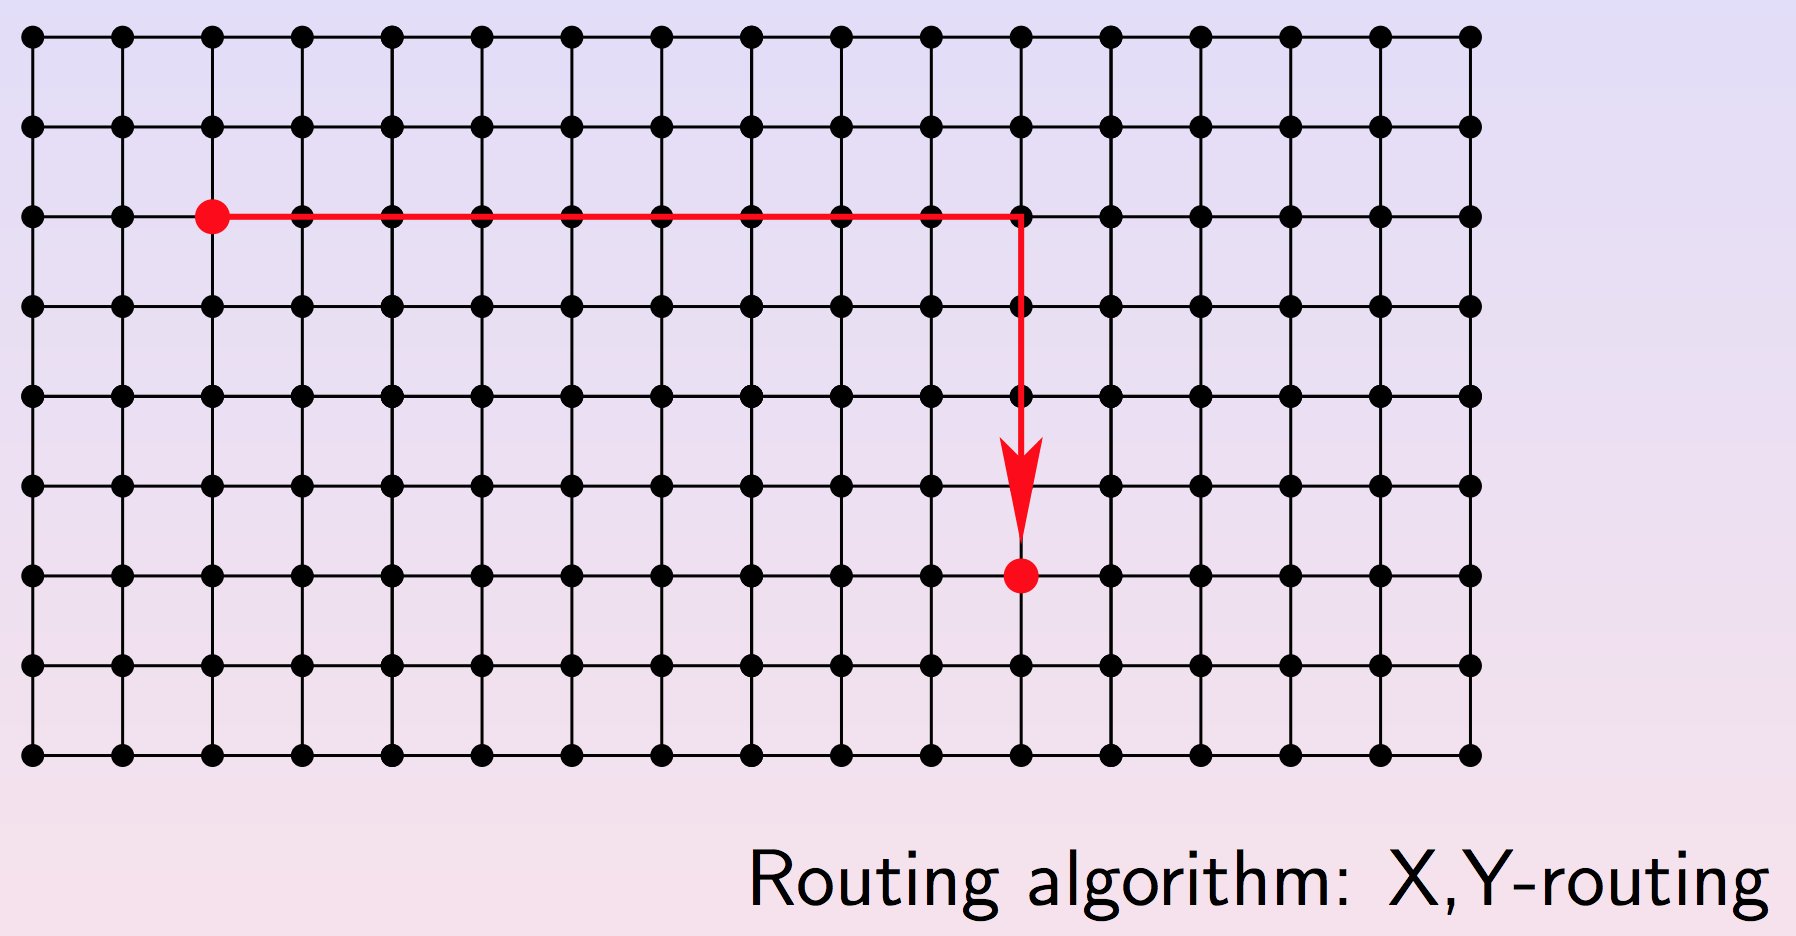
\includegraphics[scale=0.3]{images/xyrouting.png} 
    \label{fig:labeledrouting}
\end{figure}

In contract, when doing name independent routing, an adversary will label the
vertices. If the labeling is done randomly it will hold no routing information
and we can't use the label names to navigate. Thus, we need some kind of
technique to figure out what port to use for message forwarding. 

The routing scheme presented in this report is name independent.
